\subsection{Variables}

\begin{frame}{What is a Variable ?}{}
    \begin{block}{}
        A variable is a \textbf{name} that refers to a memory location.
    \end{block}
\end{frame}

\begin{frame}{Memory Location}{}
    \Huge
    \begin{itemize}
        \item Name
        \item Address (L-value)
        \item Content (R-value)
    \end{itemize}
    \pause
    \begin{center}
        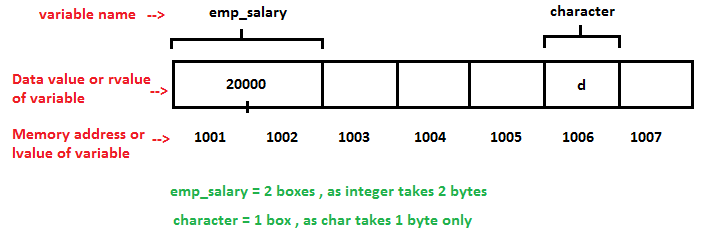
\includegraphics[height=0.4\textheight]{images/memory.png}
    \end{center}
\end{frame}

\begin{frame}[fragile]{Data Types}{}

\begin{table}[]
\centering
\Large
\begin{tabular}{|l|l|l|}
\hline
\multicolumn{1}{|c|}{\textbf{Type}} & \multicolumn{1}{c|}
    {\textbf{Keyword}} & \multicolumn{1}{c|}{\textbf{Examples}} \\ \hline
Integer                  & int       & 0, -5, 43, 6             \\ \hline
Floating point           & float     & 2.5, -0.3, 0.0012, 1.0   \\ \hline
Double Floating point    & double    & 0.5, 9.1, -0.7, 7.0      \\ \hline
\end{tabular}
\end{table}
\end{frame}

\begin{frame}[fragile]{Variable Declaration}{}
    \begin{itemize}
        \item Variable contains Garbage Value (Un-initialized)
            \begin{minted}{c++}
                int a;
            \end{minted}
    \pause
        \item Initializing with a value.
            \begin{minted}{c++}
                double b = 5.0;
            \end{minted}
    \pause
        \item Declare multiple variables
            \begin{minted}{c++}
                float a, b, c, d;
            \end{minted}
    \end{itemize}
\end{frame}

\begin{frame}[fragile]{Variable Assignment}{NOT the same as ''equals''}
    \begin{block}{} Left side is name. Right side is value. \end{block}
    {
    \Huge \begin{minted}{c++}
        a = 5;
    \end{minted}
    \begin{minted}{c++}
        b = a + 5;
    \end{minted}
    }
    \begin{block}{} We \textbf{''assign''} a value to a variable. \end{block}
\end{frame}

\begin{frame}[fragile]{Variable Assignment}{}
    \begin{center}
        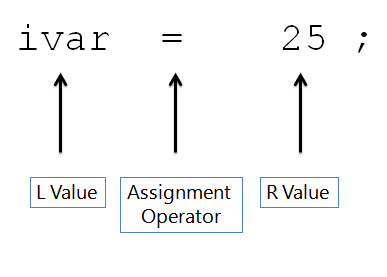
\includegraphics[height=0.4\textheight]{images/ass1.png}
    \end{center}
    \begin{center}
        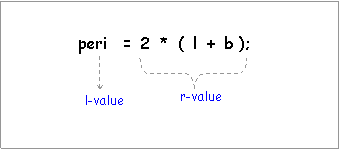
\includegraphics[height=0.4\textheight]{images/ass2.png}
    \end{center}
\end{frame}
